\documentclass[12pt,spanish,a4paper,]{article}
\usepackage{lmodern}

\usepackage{tocbasic} %% add new toc
\usepackage{floatrow}
\floatsetup[figure]{capposition=top}
\usepackage{amssymb,amsmath}
\usepackage{ifxetex,ifluatex}
\usepackage{fixltx2e} % provides \textsubscript
\ifnum 0\ifxetex 1\fi\ifluatex 1\fi=0 % if pdftex
  \usepackage[T1]{fontenc}
  \usepackage[utf8]{inputenc}
\else % if luatex or xelatex
  \usepackage{unicode-math}
  \defaultfontfeatures{Ligatures=TeX,Scale=MatchLowercase}
\fi
% use upquote if available, for straight quotes in verbatim environments
\IfFileExists{upquote.sty}{\usepackage{upquote}}{}
% use microtype if available
\IfFileExists{microtype.sty}{%
\usepackage[]{microtype}
\UseMicrotypeSet[protrusion]{basicmath} % disable protrusion for tt fonts
}{}
\PassOptionsToPackage{hyphens}{url} % url is loaded by hyperref
\usepackage[unicode=true]{hyperref}
\hypersetup{
            pdftitle={Tesis},
            pdfborder={0 0 0},
            breaklinks=true}
\urlstyle{same}  % don't use monospace font for urls
\usepackage[left=3.5cm,right=2.5cm,top=2.5cm,bottom=2.5cm]{geometry}
\ifnum 0\ifxetex 1\fi\ifluatex 1\fi=0 % if pdftex
  \usepackage[shorthands=off,main=spanish]{babel}
\else
  \usepackage{polyglossia}
  \setmainlanguage[]{spanish}
\fi
\usepackage[style=authoryear-comp,]{biblatex}
\addbibresource{references.bib}
\usepackage{longtable,booktabs}
% Fix footnotes in tables (requires footnote package)
\IfFileExists{footnote.sty}{\usepackage{footnote}\makesavenoteenv{long table}}{}
\usepackage{graphicx,grffile}
\makeatletter
\def\maxwidth{\ifdim\Gin@nat@width>\linewidth\linewidth\else\Gin@nat@width\fi}
\def\maxheight{\ifdim\Gin@nat@height>\textheight\textheight\else\Gin@nat@height\fi}
\makeatother
% Scale images if necessary, so that they will not overflow the page
% margins by default, and it is still possible to overwrite the defaults
% using explicit options in \includegraphics[width, height, ...]{}
\setkeys{Gin}{width=\maxwidth,height=\maxheight,keepaspectratio}
\IfFileExists{parskip.sty}{%
\usepackage{parskip}
}{% else
\setlength{\parindent}{0pt}
\setlength{\parskip}{6pt plus 2pt minus 1pt}
}
\setlength{\emergencystretch}{3em}  % prevent overfull lines
\providecommand{\tightlist}{%
  \setlength{\itemsep}{0pt}\setlength{\parskip}{0pt}}
\setcounter{secnumdepth}{5}

% set default figure placement to htbp
\makeatletter
\def\fps@figure{htbp}
\makeatother


\title{Tesis}

%% MONASH STUFF

%% CAPTIONS
\RequirePackage{caption}
\DeclareCaptionStyle{italic}[justification=centering]
 {labelfont={bf},textfont={it},labelsep=colon}
\captionsetup[figure]{style=italic,format=hang,singlelinecheck=true}
\captionsetup[table]{style=italic,format=hang,singlelinecheck=true}


%% FONT
\RequirePackage{bera}
\RequirePackage[charter,sfscaled]{mathdesign}
\usepackage{XCharter}
\RequirePackage{fontawesome}

%% HEADERS AND FOOTERS
\RequirePackage{fancyhdr}
\pagestyle{fancy}
\rfoot{\Large\sffamily\raisebox{-0.1cm}{\textbf{\thepage}}}
\makeatletter
\lhead{\textsf{\expandafter{\@title}}}
\makeatother
\rhead{}
\cfoot{}
\setlength{\headheight}{15pt}
\renewcommand{\headrulewidth}{0.4pt}
\renewcommand{\footrulewidth}{0.4pt}
\fancypagestyle{plain}{%
\fancyhf{} % clear all header and footer fields
\fancyfoot[C]{\sffamily\thepage} % except the center
\renewcommand{\headrulewidth}{0pt}
\renewcommand{\footrulewidth}{0pt}}

%% MATHS
\RequirePackage{bm,amsmath}
\allowdisplaybreaks

%% GRAPHICS
\RequirePackage{graphicx}
\setcounter{topnumber}{2}
\setcounter{bottomnumber}{2}
\setcounter{totalnumber}{4}
\renewcommand{\topfraction}{0.85}
\renewcommand{\bottomfraction}{0.85}
\renewcommand{\textfraction}{0.15}
\renewcommand{\floatpagefraction}{0.8}


%\RequirePackage[section]{placeins}

%% SECTION TITLES


%% SECTION TITLES
\RequirePackage[compact,sf,bf]{titlesec}
\titleformat*{\section}{\Large\sf\bfseries\color[rgb]{0,0,0}}
\titleformat*{\subsection}{\large\sf\bfseries\color[rgb]{0,0,0}}
\titleformat*{\subsubsection}{\sf\bfseries\color[rgb]{0,0,0}}
\titlespacing{\section}{0pt}{2ex}{.5ex}
\titlespacing{\subsection}{0pt}{1.5ex}{0ex}
\titlespacing{\subsubsection}{0pt}{.5ex}{0ex}


%% TITLE PAGE
\def\Date{\number\day}
\def\Month{\ifcase\month\or
 January\or February\or March\or April\or May\or June\or
 July\or August\or September\or October\or November\or December\fi}
\def\Year{\number\year}

%% LINE AND PAGE BREAKING
\sloppy
\clubpenalty = 10000
\widowpenalty = 10000
\brokenpenalty = 10000
\RequirePackage{microtype}

%% PARAGRAPH BREAKS
\setlength{\parskip}{1.4ex}
\setlength{\parindent}{0em}

%% HYPERLINKS
\RequirePackage{xcolor} % Needed for links
\definecolor{darkblue}{rgb}{0,0,.6}
\definecolor{black}{rgb}{0,0,0}
\RequirePackage{url}

\makeatletter
\@ifpackageloaded{hyperref}{}{\RequirePackage{hyperref}}
\makeatother
\hypersetup{
     citecolor=0 0 0,
     breaklinks=true,
     bookmarksopen=true,
     bookmarksnumbered=true,
     linkcolor=black,
     urlcolor=black,
     citecolor=black,
     colorlinks=black}

\usepackage[showonlyrefs]{mathtools}
\usepackage[no-weekday]{eukdate}

%% BIBLIOGRAPHY

\makeatletter
\@ifpackageloaded{biblatex}{}{\usepackage[style=authoryear-comp, backend=biber, natbib=true]{biblatex}}
\makeatother
\ExecuteBibliographyOptions{bibencoding=utf8,minnames=1,maxnames=3, maxbibnames=99,dashed=false,terseinits=true,giveninits=true,uniquename=false,uniquelist=false,doi=false, isbn=false,url=true,sortcites=false}

\DeclareFieldFormat{url}{\texttt{\url{#1}}}
\DeclareFieldFormat[article]{pages}{#1}
\DeclareFieldFormat[inproceedings]{pages}{\lowercase{pp.}#1}
\DeclareFieldFormat[incollection]{pages}{\lowercase{pp.}#1}
\DeclareFieldFormat[article]{volume}{\mkbibbold{#1}}
\DeclareFieldFormat[article]{number}{\mkbibparens{#1}}
\DeclareFieldFormat[article]{title}{\MakeCapital{#1}}
\DeclareFieldFormat[article]{url}{}
%\DeclareFieldFormat[book]{url}{}
%\DeclareFieldFormat[inbook]{url}{}
%\DeclareFieldFormat[incollection]{url}{}
%\DeclareFieldFormat[inproceedings]{url}{}
\DeclareFieldFormat[inproceedings]{title}{#1}
\DeclareFieldFormat{shorthandwidth}{#1}
%\DeclareFieldFormat{extrayear}{}
% No dot before number of articles
\usepackage{xpatch}
\xpatchbibmacro{volume+number+eid}{\setunit*{\adddot}}{}{}{}
% Remove In: for an article.
\renewbibmacro{in:}{%
  \ifentrytype{article}{}{%
  \printtext{\bibstring{in}\intitlepunct}}}

\AtEveryBibitem{\clearfield{month}}
\AtEveryCitekey{\clearfield{month}}

\makeatletter
\DeclareDelimFormat[cbx@textcite]{nameyeardelim}{\addspace}
\makeatother

\author{\sf\Large\textbf{ Karl Marx}\\ {\sf\large Filosofo, Economista, 5o semestre\\[0.5cm]} \sf\Large\textbf{ Friedrich Engels}\\ {\sf\large Filosofo, Economista, Historiador\\[0.5cm]}}

\date{23 mayo 2022}
\makeatletter
\lfoot{\sf Marx, Engels}
\makeatother


%%%% PAGE STYLE FOR FRONT PAGE OF REPORTS

\makeatletter
\def\organization#1{\gdef\@organization{#1}}
\def\telephone#1{\gdef\@telephone{#1}}
\def\email#1{\gdef\@email{#1}}
\makeatother
  \organization{Economía Política}

  \def\name{Facultad de Economía}

  \telephone{(951) 50 3 16 86}

  \email{direccion@economiauabjo.com.mx}

\def\webaddress{\url{http://buseco.monash.edu/ebs/consulting/}}
\def\logo{
\includegraphics[width=6cm]{logo}}
\def\extraspace{\vspace*{1.6cm}}
\makeatletter
\def\contactdetails{\faicon{phone} & \@telephone \\
                    \faicon{envelope} & \@email}
\makeatother

%%%% FRONT PAGE OF REPORTS
  \def\reporttype{Ensayo}

\long\def\front#1#2#3{
\newpage
\begin{singlespacing}
\thispagestyle{empty}
\vspace*{-1.4cm}
\hspace*{-1.4cm}
\hbox to 16cm{
        hola

        }
\end{singlespacing}
\newpage
}

\makeatletter
\def\titlepage{\front{\expandafter{\@title}}{\@author}{\@organization}}
\makeatother

\usepackage{setspace}
\setstretch{1.5}

%% Any special functions or other packages can be loaded here.

\usepackage{pdfpages}

\begin{document}

\DeclareNewTOC[%% Added map class
  type=mapa,
  float,
  name=Mapa,
  listname={Índice de mapas},
  ]{mapa}

\DeclareNewTOC[%% Added map class
  type=tabla,
  float,
  name=Tabla,
  listname={Índice de tablas},
  ]{tabla}


\pagenumbering{gobble}

%%%%\titlepage
%%

\includepdf{front.pdf}

\pagenumbering{Roman}

{
\setcounter{tocdepth}{2}
\tableofcontents
}
\listoftablas
\listoffigures
\listofmapas
\newpage
\pagenumbering{arabic}
\setcounter{page}{1}
\hypertarget{introducciuxf3n}{%
\section{Introducción}\label{introducciuxf3n}}

En el famoso paper, \textcite{BC64} se introdujo una familia de transformaciones \dots

\begin{figure}
\centering
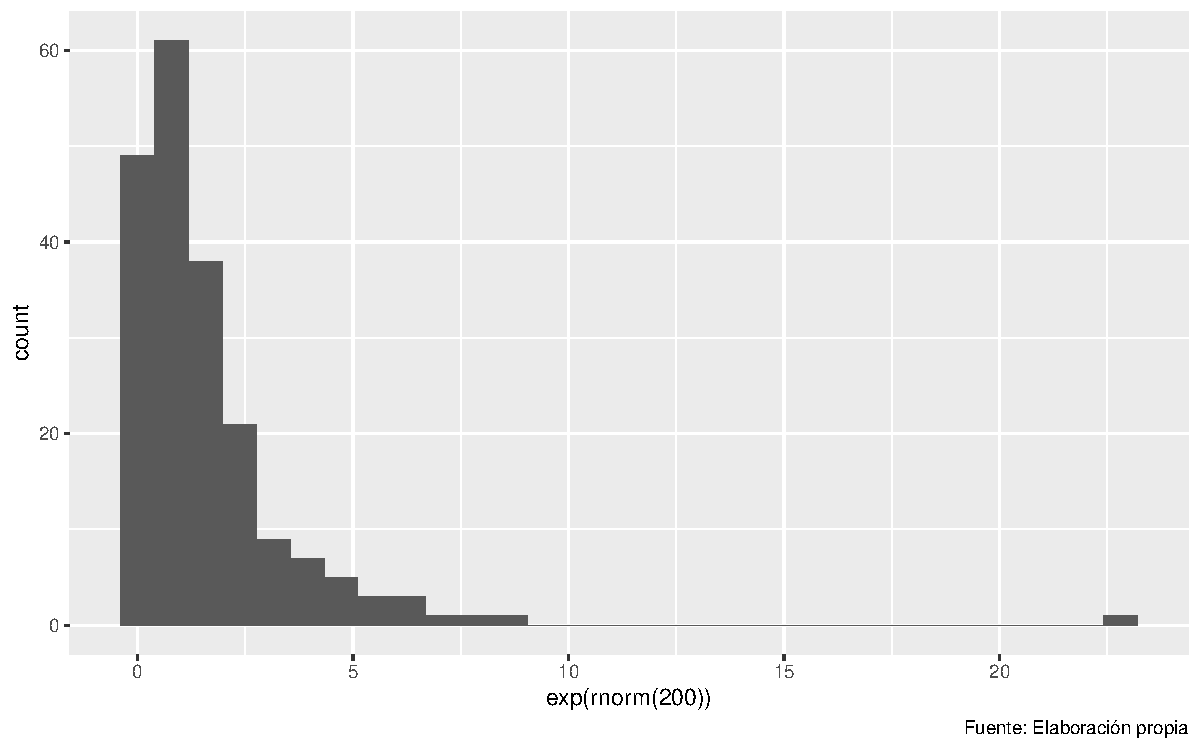
\includegraphics{skeleton_files/figure-latex/histogram-1.pdf}
\caption{\label{fig:histogram}Histograma}
\end{figure}

Considere los datos logNormal graficados en la figura \ref{fig:histogram}.

\[s^2 = \sum_{i=1}^n (x_i-\bar{x})^2\]

\hypertarget{subtema}{%
\subsection{Subtema}\label{subtema}}

Una gráfica que permite comparar una variable categórica y una numérica

\begin{figure}
\centering
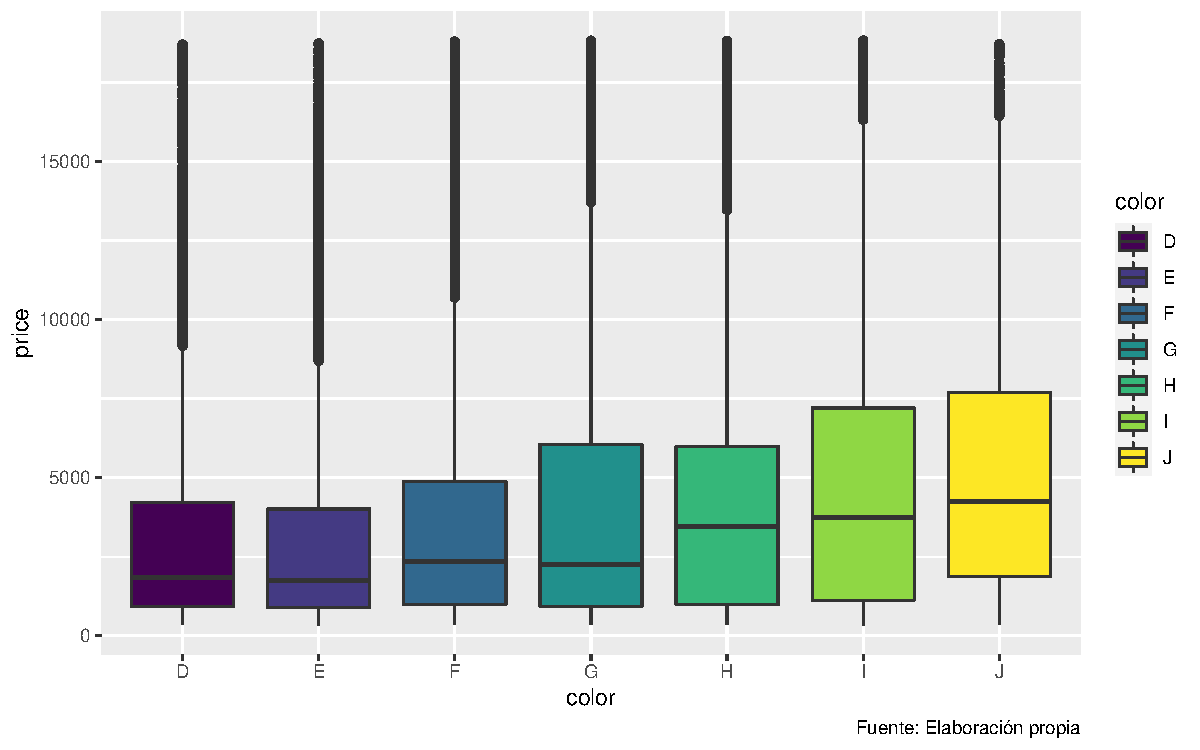
\includegraphics{skeleton_files/figure-latex/boxplot-1.pdf}
\caption{\label{fig:boxplot}Boxplot}
\end{figure}

En la figura \ref{fig:boxplot} es fácil observar los valores atípicos.

\hypertarget{desarrollo}{%
\section{Desarrollo}\label{desarrollo}}

Donec gravida vitae. Sed eros erat congue magna faucibus eu turpis tincidunt in. Varius litora vivamus, sit tempus pharetra non pretium turpis lacus. Praesent massa ornare a purus sed et. Nam justo suscipit egestas, fames quis ornare in. Metus luctus, viverra a leo porta ut purus. Et sed eget velit vitae fermentum varius, id fermentum. Nostra et enim efficitur vehicula, sit cum ultricies et.

Eu pellentesque rutrum, ligula, ultricies, eu sed interdum elementum. Platea, efficitur tortor arcu risus dis. Luctus himenaeos dolor erat praesent et. Sed sit venenatis augue ut iaculis cum, aptent rutrum odio lorem elit nisl dui. Amet a a lacinia nam eu et, sed vel aliquam inceptos. Dictum dui turpis pellentesque vel dolor dapibus tristique amet lacus sodales id nunc iaculis facilisi lacus. Sit ipsum nam eget. Nec, sed nec mauris faucibus faucibus finibus ac ut ullamcorper accumsan ligula? Finibus finibus, porttitor pellentesque fames quis non pharetra justo molestie. Lorem urna a sed lacinia. Pharetra, sit himenaeos in sagittis urna montes consectetur augue taciti eu.

\begin{mapa}
  \caption{Un mapa de diabetes.}
  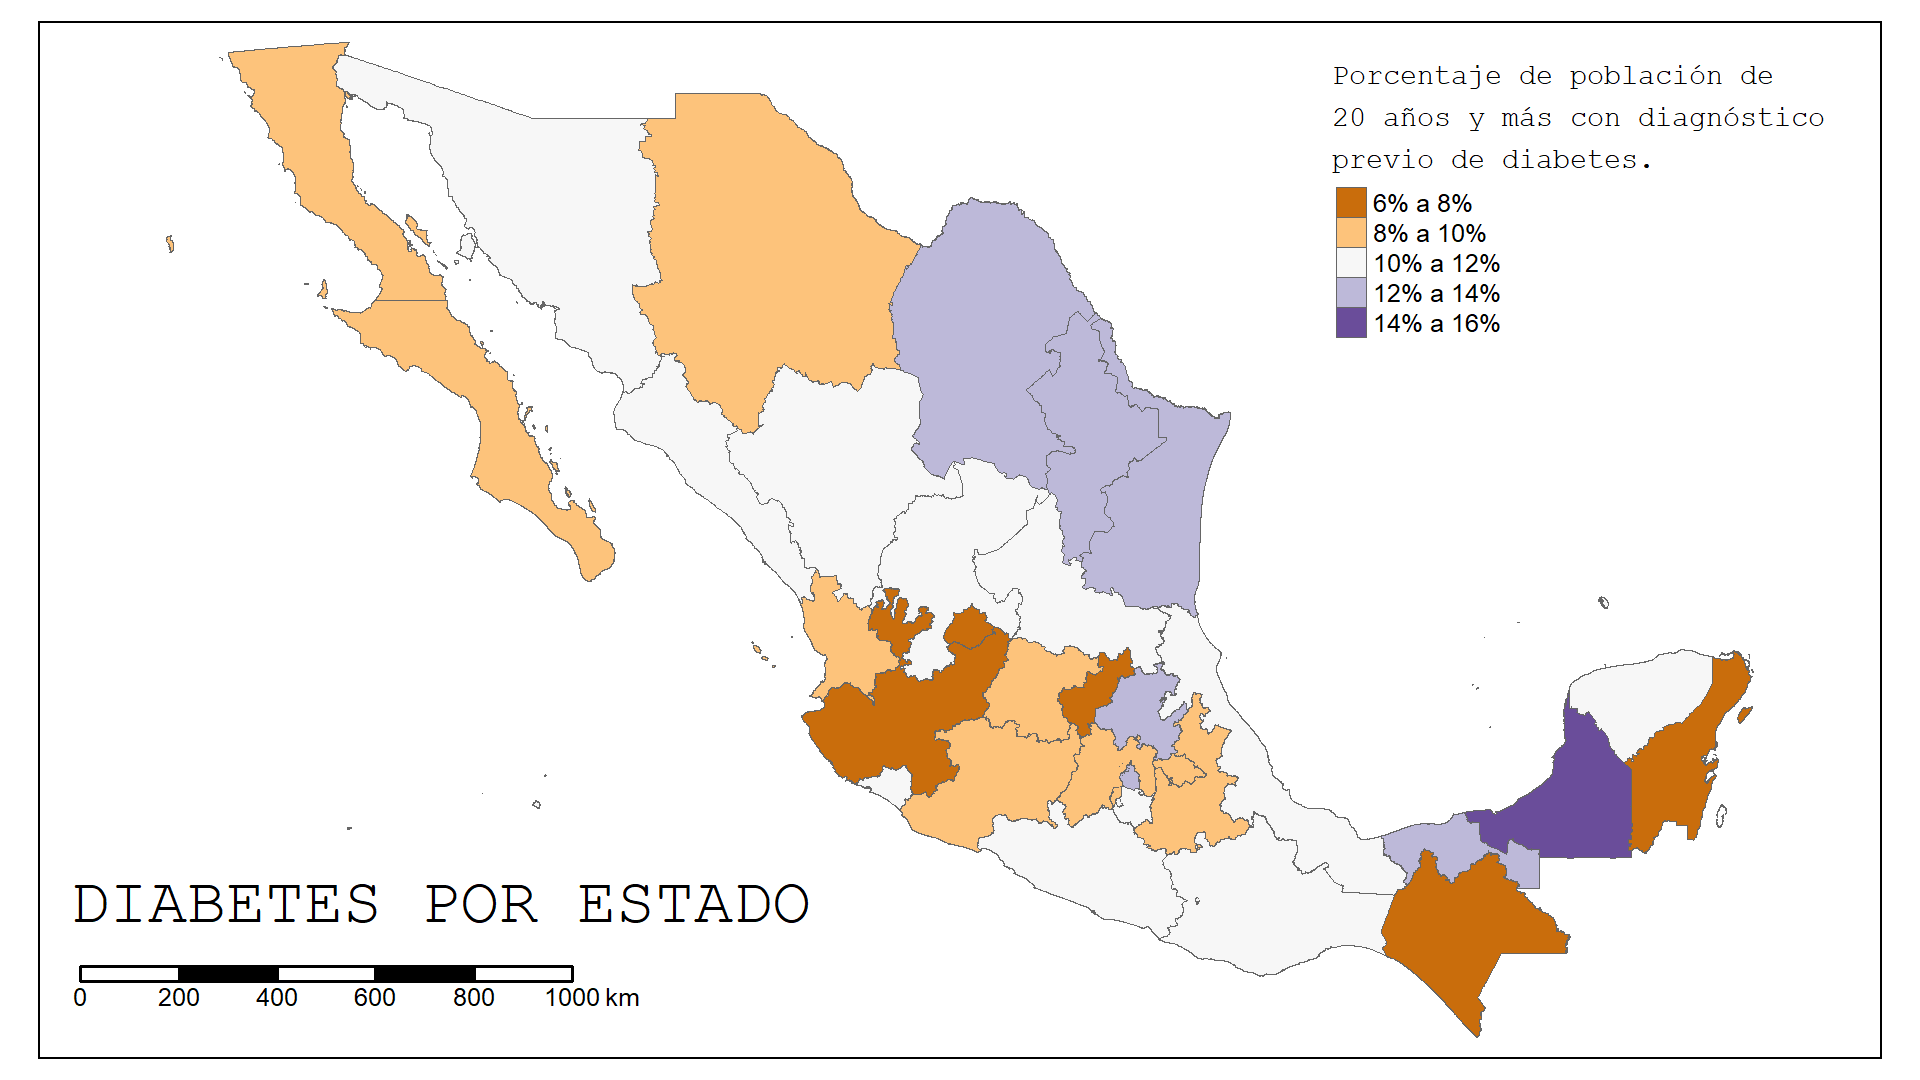
\includegraphics{images/estatal_diabetes.png}
  \footnotesize{Fuente: Elaboración propia con datos de la ENSANUT}
\end{mapa}

\begin{tabla}
  \caption{Una tabla} 
  \centering 
  \begin{tabular}{c c c c} 
  \hline\hline 
  Case & Method\#1 & Method\#2 & Method\#3 \\ 
  \hline 
  1 & 50 & 837 & 970 \\
  2 & 47 & 877 & 230 \\
  3 & 31 & 25 & 415 \\
  4 & 35 & 144 & 2356 \\
  5 & 45 & 300 & 556 \\ 
  \hline 
  \footnotesize{Fuente: Elaboración propia con datos de la ENSANUT}
  \end{tabular}
\end{tabla}

\newpage

\hypertarget{conclusiuxf3n}{%
\section{Conclusión}\label{conclusiuxf3n}}

Arcu sem condimentum taciti in ornare nascetur. Pulvinar curae vestibulum eleifend non gravida. Congue taciti non id. Sed donec in nam vitae ante ut tempor nec ante. Non curabitur sit, pellentesque laoreet ad ipsum sed, a sed, sollicitudin mattis ligula. Iaculis mauris massa. Sem proin feugiat hendrerit maximus feugiat diam eleifend facilisis, volutpat ligula tristique. Aliquam non tristique sed egestas ut ut. Semper amet ligula in metus integer. Donec fringilla turpis, et. Lacus lectus amet suscipit, et, ullamcorper aliquam.

Ornare nec vestibulum lectus. Orci urna in cras est mauris. In risus diam ac nullam sapien, eros, et enim commodo enim. Blandit eget nec tincidunt magna donec ad. Feugiat suspendisse sed malesuada velit. Pellentesque risus eros primis convallis sapien eget ridiculus etiam ante primis. Tristique turpis aptent id nec vulputate sodales, et et.

Himenaeos vivamus, imperdiet sodales in ante viverra, fermentum quis rhoncus dolor! Sit commodo ac justo volutpat velit. Mattis quisque conubia dolor convallis eros sed ex turpis eros nisi. At nostra orci non nulla condimentum malesuada himenaeos. Dictumst erat sollicitudin vehicula dolor sit et accumsan, ipsum quis sed. Tellus ultricies nisi vitae ut phasellus varius. Curabitur pretium, ac ipsum facilisis et donec, orci. Faucibus, felis sit amet est magna maximus aliquam blandit nisl tristique in porttitor magna sodales, nibh. Habitant, ultrices commodo. Egestas feugiat amet hendrerit quis malesuada ornare sed.

\newpage
\printbibliography

\end{document}
